\documentclass[a4paper,11pt]{article}
\usepackage[T1]{fontenc}
\usepackage[utf8]{inputenc}
\usepackage{lmodern}

\usepackage{graphicx}
\graphicspath{{../data/}}

\title{Image Processing 1 - Exercise 2 - WiSe 2012/13}
\author{Weipeng He}

\begin{document}

\maketitle

\begin{enumerate}
  \item If the brightness of each part of the staircase is equal, it is not possible to see the stairs. This is affected by the illumination of the scene and the sensor property of the camera.
  
  \item 
  \begin{itemize}
    \item Orignal image (B1) : \\    
    
\includegraphics[width=.6\textwidth]{B1}
    
    \item The brightness values of original image is in \texttt{data/brightness}.
    
    \item Calibrated image (B2) : \\
    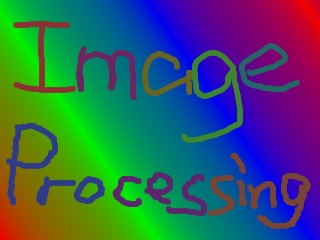
\includegraphics[width=.6\textwidth]{B2}
    
    \item Gray-scale image : \\    
    
\includegraphics[width=.6\textwidth]{B2-grayscale}
      
    \item Images are in \texttt{data/}. Source code is in \texttt{src/}.  
  \end{itemize}
  
  \item The frequency of the tv image is 25 full frames (50 half frames) per second. The interval between refreshing row 200 and row 201 is approximately half frame time, that is $ \frac{1}{50} = 0.02 s $. In this interval the car moves $ 50km/h \times 0.02s = 0.278m $, which on the screen is $ \frac{0.278}{5} \times 50 = 2.78 \approx 3 $ pixels.
\end{enumerate}

\end{document}
